\chapter{本研究の手法}
\label{method}

本章では,~\ref{approach:Hypothesis}節で述べた仮説を検証するために,本研究で行なった手法について概説する.

\section{問題解決の為のアプローチ}
\label{method:approach}
 ~\ref{approach:YotenForProblem}で述べた問題解決のための2つの要件を,本研究の手法として提案する.

 \subsection{コマンドの追加実装}
実際のShellに実装されているコマンドで,SSHの低対話型Honeypotに実装されていないコマンドを実装する.これによってコマンドの追加実装を行なった低対話型Honeypotに侵入した侵入者は,実際のShellと同じような挙動をする低対話型HoneypotをHoneypotであると検知できなくなる.

 \subsection{既実装コマンドの修正}
 SSHの低対話型Honeypotに特有の異常な挙動をする既実装コマンドを修正する.これによって既実装コマンドの修正を行なった低対話型Honeypotに侵入した侵入者は,実際のShellと同じような挙動をする低対話型HoneypotをHoneypotであると検知できなくなる.


\vspace{10mm}
\begin{figure}[H]
    \centering
    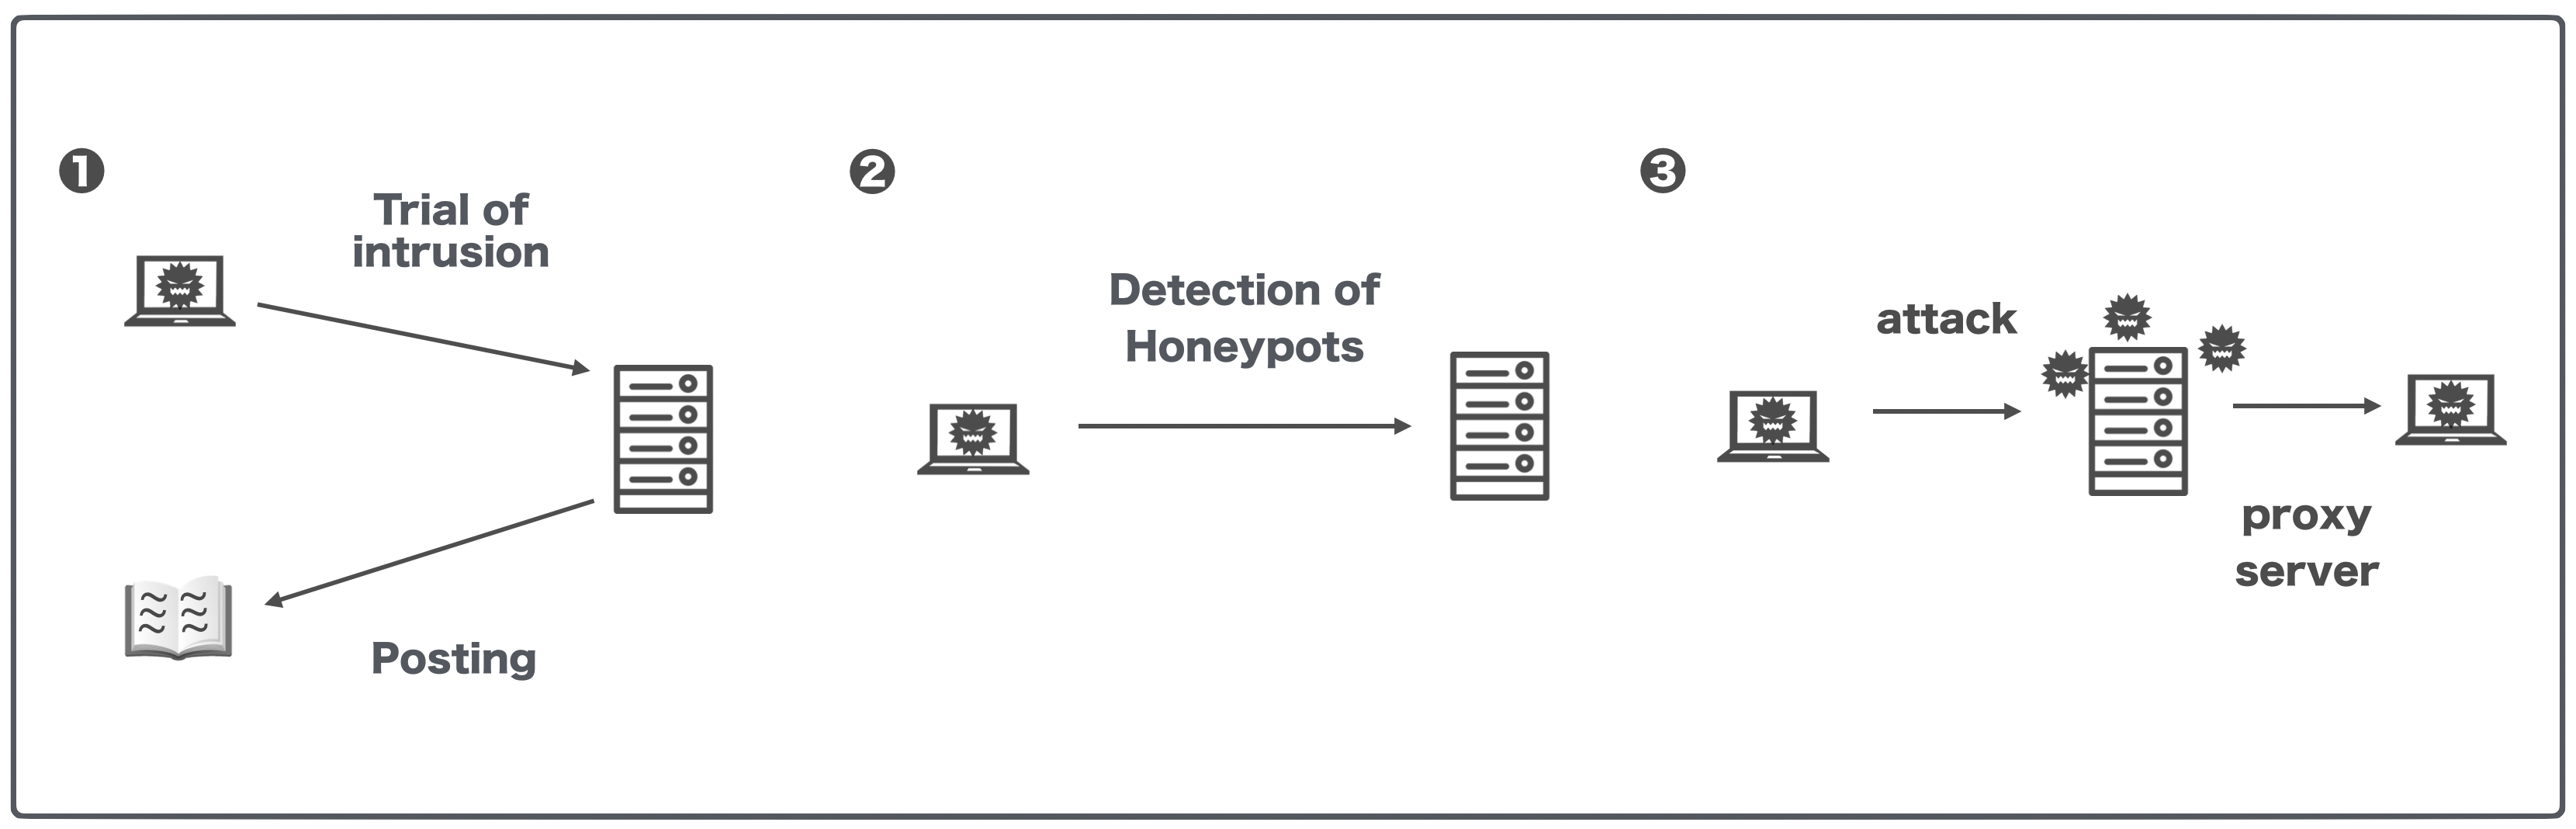
\includegraphics[width=1.0\textwidth]{figures/nagare.png}
    \caption{不正なSSH侵入者の想定行動フロー}
    \label{fig:evo}
\end{figure}
 
%%% Local Variables:
%%% mode: japanese-latex
%%% TeX-master: "../bthesis"
%%% End: